%%%%%%%%%%%%%%
% LECTURE 14 %
%%%%%%%%%%%%%%
\newpage 

\noindent \lecture{14}{22/11/2021}
\vspace{0.5cm}

\section{Fault tolerance}
Prima di discutere in dettaglio il successivo codice di correzione degli errori spendiamo alcune parole riguardanti le diverse tipologie di codici. Ne esistono di diversi esempi:
\begin{itemize}
    \item I \textbf{CSS codes} (da Calderbank-Shor-Steane), i quali generalizzano gli analoghi classici della correzione degli errori al contesto del QC;
    \item Gli \textbf{stabilizer codes}, dei quali abbiamo visto alcuni esempi nelle sezioni precedenti;
    \item Vi è il cosiddetto \textbf{toric/surface code}, il quale fornisce un approccio topologico\footnote{Si tratta di codici particolarmente ben protetti rispetto all'interazione dei qubit con l'ambiente.} al QC;
    \item E molti altri\dots
\end{itemize}
In generale esiste un'intera teoria generale riguardante questi codici, la quale evidenzia tutte le loro analogie e differenze. Si pensi ad esempio al modo con cui correggono gli errori, al numero di qubit utilizzati, ecc.

\noindent Quanto velocemente questi codici correggono gli errori? Questo è il soggetto della cosiddetta \textbf{fault tolerance} in QC (esiste un analogo classico), perché quando si ha un errore bisogna essere certi di non averne troppi (nel senso che sono talmente tanti da non poter essere corretti in un tempo ragionevole) e inoltre bisogna assicurarsi che i circuiti non possiedano gate che propaghino questi errori. Anche in questo caso esiste ua teoria generale riguardante il come costruire circuiti quantistici che siano ottimizzati per la correzione degli errori. 

\noindent La logica della fault tolerance è la seguente: si fissa un probabilità $p$ che un qualche elemento del circuito non svolga correttamente il proprio lavoro (si pensi ad esempio alla probabilità di fallimento di un filo o un gate) e, data $p$, si vuole conoscere quanti qubit aggiuntivi è necessario introdurre per correggere tutti questi errori. In generale si fissa una soglia, la quale non è altro che la probabilità che il circuito fornisca l'output desiderato: lo scopo è quello di bilanciare opportunamente le componenti del circuito affinché esso lavori al di sotto di tale soglia. Più precisamente: il fine ultimo è quello di conoscere la probabilità che un singolo componente del circuito fallisca; in questo modo, con un numero polinomiale di qubit extra, si possono correggere gli errori avendo la certezza che il risultato sia corretto a meno di una soglia fissata. In generale, i codici fault tolerant sono quelli in cui si introducono un ragionevole ammontare di componenti extra senza modificare l'efficienza e la velocità di esecuzione dei codici. 

\noindent Non entreremo nel dettaglio, tuttavia è bene ricordare ciò che sottolineammo nella Sottosezione \ref{subsec:quantum_gates}: l'insieme di gate $\{ H, T, S, \texttt{CNOT} \}$ è universale sebbene $S$ e $T$ non siano indipendenti perché $S= \sqrt{Z}$ e $T = \sqrt{S}$; nonostante $S$ sembri ridondante nella descrizione, affinché si abbia un codice fault tolerant è necessario tenere in considerazione anche questo gate. 

\section{Toric code}
L'ultimo esempio che analizziamo di codice di correzione degli errori è il cosiddetto \textbf{toric code} (conosciuto con questo nome nella letteratura della fisica della materia condensata), detto anche più genericamente \textbf{surface code}. È un codice peculiare per diverse ragioni: innanzitutto, dal punto di vista della correzione degli errori, è un codice fault tolerant perché è molto "robusto" contro gli errori; in secondo luogo è molto interessante perché è legato ad altre branche della fisica oltre al QC: si tratta di un esempio di una situazione in cui appare una fase topologica non banale della materia e, per tale motivo, è stato in passato uno dei modelli che ha condotto all'idea della cosiddetta \textbf{topological quantum computing}. Dal nostro punto di vista è interessante per la correzione degli errori e per l'approccio topologico al QC. 

\noindent Come mostra la Figura \ref{subfig:Toric_lattice_1}, consideriamo un reticolo $L \times L$ di qubit in cui questi ultimi "vivono" sui link (collegamenti) del reticolo (si vedano i puntini rossi sui lati dei quadrati). Dal punto di vista pratico si costruisce un array periodico di qubit su un reticolo. Dato che sono presenti 2 qubit indipendenti per ogni faccia (assumiamo il qubit a sinistra e in basso nei diversi quadrati) allora la dimensione dello spazio di Hilbert totale non è altro che
\begin{equation*}
    \dim \mathcal{H} = 2^n = 2^{2 L^2} \, ,
\end{equation*}
dove $L^2$ è il numero di link/facce (si hanno $L$ righe e $L$ colonne). Quindi in totale avremo $n = 2 L^2$ qubit indipendenti. In generale questo codice funziona molto bene quando si ha un grande numero di qubit.

\begin{figure}[!h]
	\centering	
	\subfloat[][Reticolo di qubit.\label{subfig:Toric_lattice_1} ]{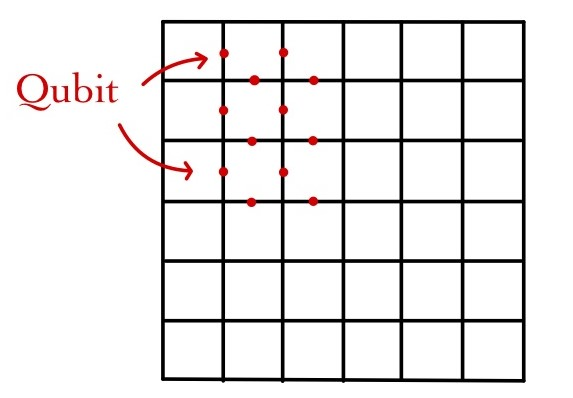
\includegraphics[scale=.43,keepaspectratio]{images/Toric_lattice_1}} \quad
	\subfloat[][Operatore $A_v$.\label{subfig:Toric_lattice_2} ]{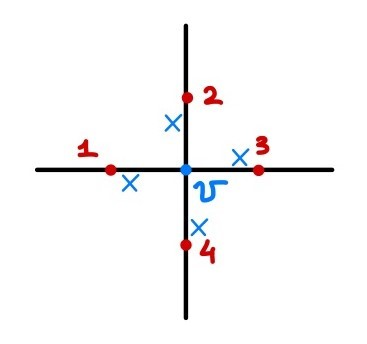
\includegraphics[scale=.43,keepaspectratio]{images/Toric_lattice_2}} \quad 
	\subfloat[][Operatore $B_p$.\label{subfig:Toric_lattice_3} ]{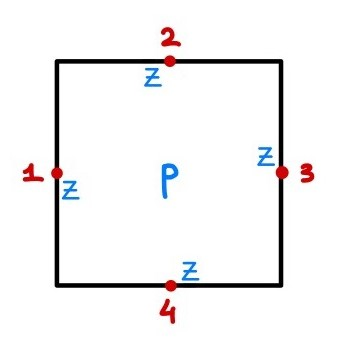
\includegraphics[scale=.43,keepaspectratio]{images/Toric_lattice_3}}
	\caption{\eqref{subfig:Toric_lattice_1} Reticolo $L \times L$ costituito da $2L^2$ qubit indipendenti. Per ogni plaquette ci sono 2 qubit indipendenti, quello in basso e quello a sinistra. \eqref{subfig:Toric_lattice_2} L'operatore rappresentato è esplicitamente $A_v = X_1 X_2 X_3 X_4$. \eqref{subfig:Toric_lattice_3} L'operatore rappresentato è esplicitamente $B_p = Z_1 Z_2 Z_3 Z_4$.}
    \label{fig:Toric_lattice}
\end{figure}

\noindent Il codice fu proposto per la prima volta dal fisico Alexei Kitaev ed è realizzato su un reticolo con condizioni al bordo periodiche (PBC: Periodic Boundary Conditions): dal punto di vista topologico considerare PBC sul quadrato di Figura \ref{subfig:Toric_lattice_1} significa porre il reticolo di qubit su un \textbf{toro} (il reticolo è bidimensionale, ma il volume è tridimensionale). Per realizzazioni concrete il toro risulta tuttavia poco pratico: in realtà la fisica del codice può essere ben rappresentata anche mediante strutture planari con opportune condizioni al bordo (per tale motivo il codice è anche detto \textbf{surface code}); anche l'idea di realizzazione di questa procedura su strutture planari fu proposta da Kitaev.

\noindent Ancora una volta la logica del codice è la stessa di quelle viste nelle precedenti sezioni perché è un \textbf{stabilizer code}. Vi sono due tipologie di stabilizers: per ogni vertice $v$ del reticolo si costruisce un operatore $A_v$ dato dal prodotto degli \texttt{X-gate} di ogni link appartenente al vertice e, similmente, per ogni faccia $p$ del reticolo (detta \textbf{plaquette}) si definisce l'operatore $B_p$ come prodotto dei 4 \texttt{Z-gate} sui link della plaquette. Si faccia riferimento alle Figure \ref{subfig:Toric_lattice_2} e \ref{subfig:Toric_lattice_3} per una rappresentazione grafica di questi operatori (chiaramente, così come i qubit, anche i gate si trovano sui link del reticolo). Dal punto di vista degli operatori avremo 
\begin{equation}\label{A_B}
    A_v = \prod_{j \in v} X_j \, , \qquad B_p = \prod_{j \in p} Z_j \, .
\end{equation}
In totale si hanno $L^2$ differenti operatori $A_v$ (uno per ognuno degli $L^2$ vertici) e $L^2$ differenti operatori $B_p$ (uno per ognuna delle $L^2$ plaquette): abbiamo quindi $2L^2$ differenti stabilizers. L'idea è, come al solito negli stabilizer codes, quello di codificare i qubit logici nel sottospazio (dato un certo autovalore) di questo insieme di operatori: più precisamente sappiamo che possiamo codificare il codewords nell'autospazio comune di questi operatori se commutano tra loro e il loro quadrato è l'identità. È evidente che per ogni $v$ e $p$, in quanto prodotto di matrici di Pauli, avremo $A^2_v = B^2_p = \mathbb{I}$. Inoltre si ha
\begin{equation}\label{commutatori_A_B}
    \comm{A_v}{B_p} = 0 \, , \qquad \comm{A_v}{A_{v'}} = 0 \, , \qquad \comm{B_p}{B_{p'}} = 0 \, \, \quad \forall \, v,p,v',p' \, ;
\end{equation}
il secondo e il terzo commutatore sono banali, tuttavia il primo è meno ovvio. Chiaramente questo commutatore è nullo quando $A_v$ e $B_p$ agiscono su qubit diversi (vertice e plaquette disgiunti), tuttavia potrebbe non essere nullo nel caso in cui $A_v$ sia localizzato in uno dei quattro vertici di una plaquette $p$ (si pensi al vertice \ref{subfig:Toric_lattice_2} posto su uno dei quattro vertici della plaquette \ref{subfig:Toric_lattice_3}): nonostante questa situazione, le matrici $X$ e $Z$ che agiscono sui qubit di un medesimo sottospazio sono sempre 2. Questo significa che i due anticommutatori $\acomm{Z_i}{X_i} = 0$ producono $(-1)^2 = 1$, quindi anche in questo caso il primo commutatore è dimostrato. 

\noindent Possiamo definire come codewords il sottospazio di $\mathcal{H}$ corrispondente all'autospazio comune agli operatori $A_v$ e $B_p$ con autovalore $+1$, ossia
\begin{equation*}
    C = \{ \text{Sottospazio comune agli operatori con autovalore } A_v = B_p = +1 \} \, .
\end{equation*}
Qual è la dimensione di $C$? Ricordando dalla \eqref{A_B} che gli stabilizers sono prodotti di matrici di Pauli, essi "tagliano" sempre $\mathcal{H}$ in due sottospazi della medesima dimensione: dato che abbiamo $L^2$ operatori $A_v$ e $L^2$ operatori $B_p$ allora si ha $\dim C = 2^{2L^2}/2^{L^2}/2^{L^2} = 1$, quindi sembrerebbe che non possiamo codificare i qubit in $C$. Il problema è che ci siamo dimenticati che non tutti questi stabilizers sono indipendenti! Essi soddisfano infatti
\begin{equation}\label{constraint_A_B}
    \prod_v A_v = \mathbb{I} \, , \qquad \prod_p B_p = \mathbb{I} \, ;
\end{equation}
queste proprietà derivano dal fatto che nei prodotti di tutti i possibili vertici e plaquette ci sono sempre almeno 2 matrici di Pauli in comune tali che $X_i^2 = \mathbb{I}$ e $Z_i^2 = \mathbb{I}$. Si pensi ad esempio all'operatore $A_{v_1}$ della Figura \ref{subfig:Toric_lattice_2} adiacente ad un altro $A_{v_2}$, i quali hanno un link in comune e quindi gli \texttt{X-gate} di quel link daranno $X^2 = \mathbb{I}$; discorso simile per due plaquette adiacenti $B_{p_1}$ e $B_{p_2}$ della Figura \ref{subfig:Toric_lattice_3}, le quali hanno un link comune che darà $Z^2 = \mathbb{I}$. I vincoli \eqref{constraint_A_B} fanno sì che si abbiano in totale  $(L^2-1) + (L^2-1)$ operatori $A_v$ e $B_p$ indipendenti: dunque il codewords ha dimensione 
\begin{equation*}
    \dim C = 2^{2 L^2} / 2^{L^2-1} / 2^{L^2-1} = 4 \, .
\end{equation*}
Questo significa che nel toro  possiamo codificare fino a 4 stati logici, ovvero 2 qubit logici. In realtà nel caso planare  si ha $\dim C = 2$, quindi possiamo codificare un singolo qubit logico (come nei codici precedenti). 

\noindent Come costruiamo gli stati logici del codewords $C$? Possiamo procedere in maniera esattamente analoga al caso di Steane: partiamo dallo stato $\ket{000 \ldots 0}$ (prodotto tensoriale dei $2L^2$ qubit indipendenti del reticolo) e calcoliamo 
\begin{equation}\label{logical_00}
    \ket{\overline{00}} = \prod_v \frac{(\mathbb{I}+A_v)}{\sqrt{2}} \ket{000 \ldots 0} \, ;
\end{equation}
sappiamo che in questo modo otteniamo automaticamente un autostato di qualsiasi $A_v$ con autovalore $+1$ perché $A_v (\mathbb{I} + A_v) \ket{\psi} = (A_v + \mathbb{I}) \ket{\psi}$. Analogamente avremo che $\ket{\overline{00}}$ è anche autostato di ogni $B_p$ con autovalore $+1$ perché valgono i commutatori \eqref{commutatori_A_B} e perché $B_p$ è un prodotto di \texttt{Z-gate} ($Z \ket{0} = \ket{0}$):
\begin{equation*}
    B_p (\mathbb{I} + A_v) \ket{000 \ldots 0} = (\mathbb{I} + A_v) B_p \ket{000 \ldots 0} = (\mathbb{I} + A_v) \ket{000 \ldots 0} \, .
\end{equation*}
In aggiunta allo stato $\ket{\overline{00}}$, dato che $\dim C = 4$, ci sono altri 3 stati logici che chiamiamo $\ket{\overline{01}}$, $\ket{\overline{10}}$ e $\ket{\overline{11}}$. Al posto che costruirli scrivendo formule analoghe alla \eqref{logical_00} possiamo identificare degli opportuni operatori logici $\overline{X}_1$, $\overline{X}_2$, $\overline{Z}_1$ e $\overline{Z}_2$ tali che permettano di costruire questi ultimi a partire da $\ket{\overline{00}}$: $\overline{X}_1 \ket{\overline{00}} = \ket{\overline{10}}$, ecc. Come riferimento grafico per la discussione che segue si vedano i due reticoli di Figura \ref{fig:logical_X_Z}.   

\begin{figure}[!h]
	\centering	
	\subfloat[][Operatori logici $\overline{Z}_1$ e $\overline{Z}_2$.\label{subfig:logical_X_Z_1} ]{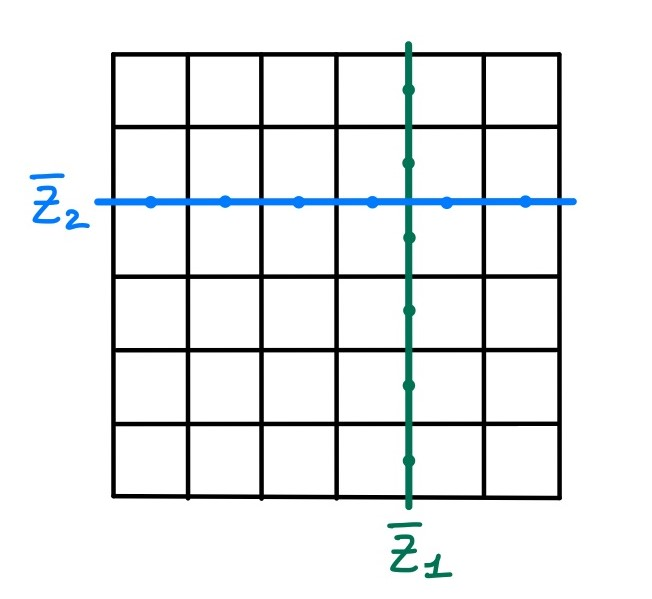
\includegraphics[scale=.43,keepaspectratio]{images/logical_X_Z_1}} \quad
	\subfloat[][Operatori logici $\overline{X}_1$ e $\overline{X}_2$.\label{subfig:logical_X_Z_2} ]{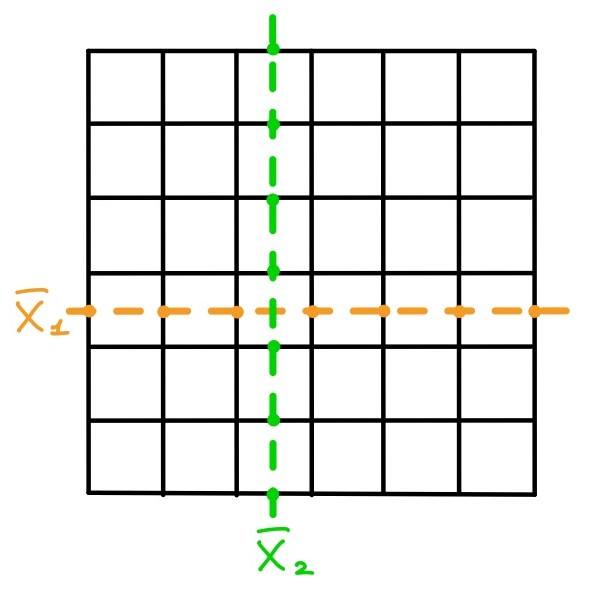
\includegraphics[scale=.43,keepaspectratio]{images/logical_X_Z_2}} 
	\caption{Le linee che rappresentano gli operatori logici $\overline{Z}_1$, $\overline{Z}_2$, $\overline{X}_1$ e $\overline{X}_2$ non sono altro che linee chiuse grazie alle PBC, quindi sono loop attorno al reticolo toroidale. I pallini rappresentati in corrispondenza dei link indicano i singoli gate che costituiscono il prodotto di quell'operatore logico.}
    \label{fig:logical_X_Z}
\end{figure}

\noindent Come mostrato nella Figura \ref{subfig:logical_X_Z_1}, definiamo $\overline{Z}_1$ come il prodotto di tutti gli \texttt{Z-gate} individuati dall'intersezione della linea verticale passante per i link del reticolo; similmente $\overline{Z}_2$ è definito come il prodotto degli \texttt{Z-gate} individuati dall'intersezione della linea orizzontale passante per i link. Esplicitamente avremo
\begin{equation}\label{logical_Z_1_2}
    \overline{Z}_1 = \prod_{i \in \text{vline}} Z_i \, , \qquad \overline{Z}_2 = \prod_{i \in \text{hline}} Z_i \, ,
\end{equation}
dove le diciture "vline" e "hline" indicano rispettivamente la linea verticale e la linea orizzontale passante per i link del reticolo. 

\noindent Similmente agli operatori \eqref{logical_Z_1_2} consideriamo ora la Figura \ref{subfig:logical_X_Z_2}. Se consideriamo questa volta il \textbf{reticolo duale}, ossia l'analogo reticolo che si costruisce passando per i punti medi dei link del reticolo di partenza, possiamo definire $\overline{X}_2$ come prodotto degli \texttt{X-gate} intercettati dalla linea verticale passante per il reticolo duale; infine definiamo $\overline{X}_1$ come prodotto degli \texttt{X-gate} intercettati dalla linea orizzontale passante per il reticolo duale. In termini di operatori scriviamo
\begin{equation}\label{logical_X_1_2}
    \overline{X}_1 = \prod_{i \in \text{hline}} X_i \, , \qquad \overline{X}_2 = \prod_{i \in \text{vline}} X_i \, ,
\end{equation}
dove questa volta le diciture "hline" e "vline" indicano rispettivamente la linea orizzontale e la linea verticale passante per i link del reticolo duale. È importante notare che grazie alle PBC le linee degli operatori $\overline{Z}_1$, $\overline{Z}_2$, $\overline{X}_1$ e $\overline{X}_2$ rappresentate nella Figura \ref{fig:logical_X_Z} non sono altro che \textbf{loop} (linee chiuse) passanti attorno al reticolo toroidale. D'ora in avanti ci riferiremo a queste linee chiamandole equivalentemente con il termine "loop".  

\noindent Come possiamo essere certi che gli operatori \eqref{logical_Z_1_2} e \eqref{logical_X_1_2} siano i corretti operatori logici? Sappiamo che gli operatori logici agiscono sul sottospazio $C$ e producono un nuovo stato $\ket{\psi} \in C$; questo significa che se gli operatori appena definiti commutano con tutti gli $A_v$ e $B_p$ allora la loro azione su stati del codewords produce altri stati di $C$, altrimenti, se anticommutano con $A_v$ e $B_p$, la loro azione su $C$ produce nuovi stati non più facenti parte del codewords, ossia si tratta di operatori corrispondenti ad errori. In altre parole dobbiamo quindi verificare che per ogni $i = 1 ,2$ e per qualsiasi $v$ e $p$ avremo
\begin{align}
    \comm{ \,\overline{X}_i}{ A_v} &= 0 \, , &\comm{ \,\overline{Z}_i}{ B_p} &= 0 \label{comm_log_banali} \\
    \comm{ \,\overline{X}_i}{ B_p} &= 0 \, , &\comm{ \,\overline{Z}_i}{ A_v} &= 0 \, . \label{comm_log_meno_banali}
\end{align}
Chiaramente, ricordando le definizioni \eqref{A_B}, le \eqref{comm_log_banali} sono banali. Per quanto riguarda invece le \eqref{comm_log_meno_banali} il discorso è più sottile: se si considerano operatori $A_v$ (vertici di Figura \ref{subfig:Toric_lattice_2}) e $B_p$ (plaquette di Figura \ref{subfig:Toric_lattice_3}) disgiunti rispetto alle linee individuate rispettivamente da $\overline{Z}_i$ e $\overline{X}_i$ allora i commutatori sono ancora una volta banali. Se si considera tuttavia un vertice $A_v$ sulla linea $\overline{Z}_i$ allora esso presenterà alcuni operatori agenti sul medesimo sottospazio di quelli del loop: gli \texttt{X-gate} di $A_v$ sul loop $\overline{Z}_i$ saranno sempre due (sopra e sotto per $\overline{Z}_1$ e destra e sinistra per $\overline{Z}_2$), quindi come per \eqref{commutatori_A_B}, le due anticommutazioni producono $(-1)^2 = +1$ e il commutatore è dimostrato. Vale un discorso analogo per gli operatori $B_p$: quando la plaquette di $B_p$ si interseca con una delle due linee $\overline{X}_i$ allora saranno sempre e solamente 2 gli \texttt{Z-gate} di $B_p$ agenti sul medesimo sottospazio degli \texttt{X-gate} del loop $\overline{X}_i$ (sopra e sotto per $\overline{X}_2$ e destra e sinistra per $\overline{X}_1$); perciò le due anticommutazioni producono come prima $(-1)^2 = +1$ e il commutatore è verificato\footnote{Per capire ancora meglio questo discorso si provi a sovrapporre gli operatori $A_v$ e $B_p$ delle Figure \ref{subfig:Toric_lattice_2} e \ref{subfig:Toric_lattice_3} con le linee delle Figure \ref{subfig:logical_X_Z_1} e \ref{subfig:logical_X_Z_2} rispettivamente: apparirà evidente come sono sempre due gli operatori anticommutanti agenti sul medesimo sottospazio.}.

\noindent Affinché $\overline{Z}_1$, $\overline{Z}_2$, $\overline{X}_1$ e $\overline{X}_2$ siano i corretti operatori logici non solo devono essere verificati i commutatori sopra, ma inoltre deve valere
\begin{equation*}
    \acomm{\overline{X}_1}{\overline{Z}_1} = 0 \, , \qquad \acomm{\overline{X}_2}{\overline{Z}_2} = 0 \, ;
\end{equation*}
queste relazioni sono ovvie se si pensano ai loop di Figura \ref{fig:logical_X_Z}: nell'intersezione di $\overline{X}_1$ con $\overline{Z}_1$ e di $\overline{X}_2$ con $\overline{Z}_2$ vi è precisamente un solo operatore ($X$ per $\overline{X}_i$ e $Z$ per $\overline{Z}_i$) che agisce sul medesimo sottospazio comune perché l'intersezione tra le due linee avviene in un solo punto. Questo fatto fa in modo che grazie all'anticommutatore $\acomm{X}{Z} = 0$ gli anticommutatori logici precedenti siano anch'essi verificati.  

\noindent Dati quindi gli operatori logici in \eqref{logical_Z_1_2} e \eqref{logical_X_1_2} possiamo calcolare i 3 stati logici rimanenti ($\ket{\overline{01}}$, $\ket{\overline{10}}$ e $\ket{\overline{11}}$) a partire dallo stato \eqref{logical_00}. Nonostante ciò qui si evidenzia la natura topologica del codice: avremmo potuto proporre come operatori logici moltissimi altri loop oltre alle linee di Figura \ref{fig:logical_X_Z}, ma ciò non avrebbe fatto alcuna differenza perché si tratta sempre di loop omotopi a quelle linee!

\noindent Il motivo profondo dell'affermazione precedente è mostrato nell'esempio di Figura \ref{fig:topological_loops}. 

\begin{figure}[!ht]
    \centering
    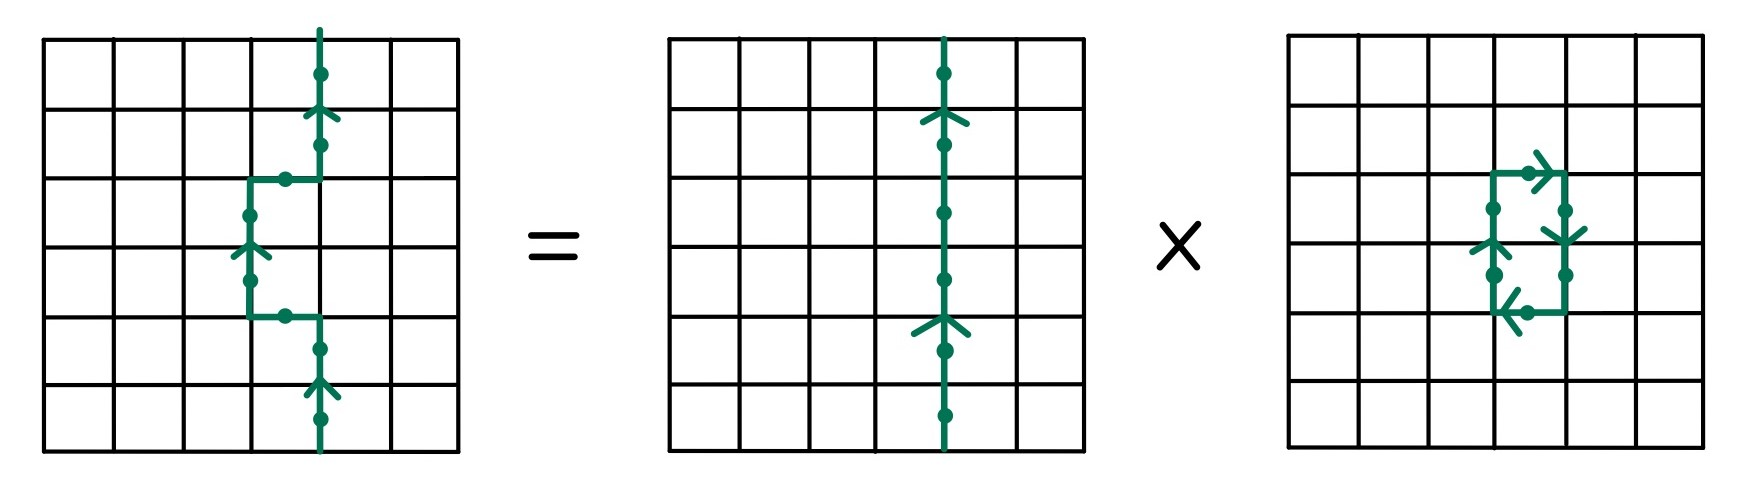
\includegraphics[scale=0.33]{images/topological_loops}
    \caption{Una possibile scelta di operatore logico $\overline{Z}_1$ è dato dal loop spezzato a sinistra. Questo loop è in realtà equivalente al loop dritto della Figura \ref{subfig:logical_X_Z_1} per il loop chiuso a destra, il quale è omotopo a zero, ossia all'identità quando agisce sul codewords.}
    \label{fig:topological_loops}
\end{figure}

\noindent Nella parte sinistra della figura è presentato un esempio di scelta differente di $\overline{Z}_1$, il quale non è altro che un loop (linea) lungo il toro che non è più dritto. Si può infatti dimostrare con argomenti analoghi ai precedenti che è un operatore logico $\overline{Z}_1$ perché soddisfa i commutatori \eqref{comm_log_banali} e \eqref{comm_log_meno_banali}.  Sembrerebbe da questa scelta che possiamo avere un'infinità di loop analoghi, tuttavia ora dimostriamo che in realtà il loop a sinistra è equivalente al prodotto del loop dritto al centro della Figura \ref{fig:topological_loops} (ossia quello della Figura \ref{subfig:logical_X_Z_1}) per il loop chiuso a destra, dove quest'ultimo è dato dal prodotto di tutti gli \texttt{Z-gate} lungo tale loop. Per capire questo fatto consideriamo il loop chiuso a destra: con la stessa logica possiamo pensare a questo loop, che circonda due plaquette, come al prodotto dei due loop più piccoli che circondano ciascuno una singola plaquette. In tale situazione il link orizzontale intermedio comune ai due loop conta 2 operatori $Z$, ciascuno da uno dei due loop: grazie alla proprietà $Z^2 = \mathbb{I}$ allora effettivamente questo loop attorno alle due plaquette è equivalente al prodotto dei due loop singoli. 

\noindent Quale sarà il loop più piccolo possibile? Chiaramente questo non è altro che il prodotto di 4 \texttt{Z-gate} attorno ad una plaquette, ossia, dalla definizione \eqref{A_B}, proprio lo stabilizer $B_p$ di Figura \ref{subfig:Toric_lattice_3}; ma ricordiamo che ciascun $B_p$ sul codewords ha autovalore $+1$! Questo significa che ciascun loop non dritto del reticolo è equivalente ad un loop dritto (Figura \ref{subfig:logical_X_Z_1}) grazie al fatto che ogni loop chiuso abbia un contributo banale su $C$: 2 loop omotopi sono equivalenti quando agiscono sul codewords! È questo il motivo fondamentale per cui il codice è chiamato \textbf{topologico}: è possibile deformare i contorni di $\overline{Z}_i$ e $\overline{X}_i$ senza cambiare l'azione di questi operatori logici sugli stati del codewords!

\noindent Notiamo che con la stessa logica precedente un qualsiasi prodotto di \texttt{Z-gate} lungo un loop chiuso contraibile è equivalente all'identità quando agisce su $C$:
\begin{equation}\label{product_Z_closed_loop}
    \prod_{i \in \substack{\text{loop} \\ \text{chiuso}\\ \text{contraibile}}} Z_i \equiv \mathbb{I} \, \text{ agendo su } C \, .
\end{equation}
Perciò il contributo del prodotto precedente è banale su $C$ perché un qualsiasi loop chiuso può essere decomposto come prodotto di plaquette singole, ossia come prodotto di $B_p$, le quali hanno autovalore $+1$ sul codewords. Questo fatto può essere espresso in altre parole dicendo che qualsiasi loop chiuso contraibile sia omotopo a zero, ossia è equivalente all'azione dell'identità sul codewords. 

\noindent Qual è quindi la ragione per cui abbiamo esattamente 4 operatori logici non banali? Il motivo è che qualsiasi operatore non banale sul toro deve essere periodico: i due loop della Figura \ref{fig:torus} (ricordare che sono prodotti di operatori), a differenza di qualsiasi altro loop, non sono omotopi a zero e ciascuno dei due può essere costituito dal prodotto di \texttt{Z-gate} oppure \texttt{X-gate}. Abbiamo quindi in totale 4 operatori non banali (2 loop non-contraibili con prodotti di $Z$ più 2 loop con prodotti di $X$). 

\begin{figure}[!h]
    \centering
    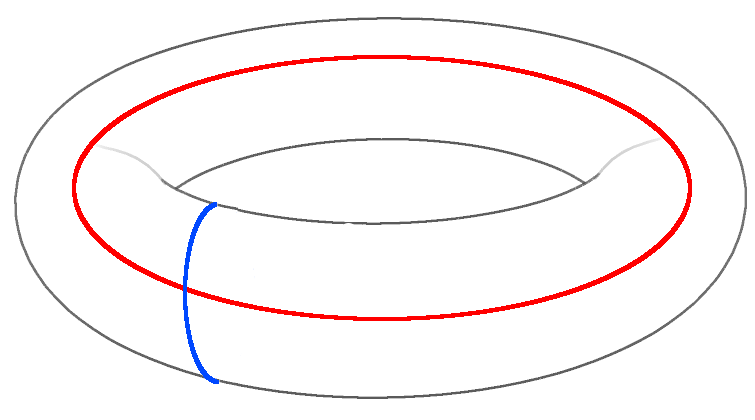
\includegraphics[scale=0.33]{images/torus}
    \caption{Abbiamo in totale 4 operatori logici non banali: 2 loop rossi e 2 loop blu . Ogni tipologia di loop (rosso o blu) può essere originata da prodotti di \texttt{Z-gate} o \texttt{X-gate}. Qualsiasi altro loop non rappresentato in figura è banale, ossia è omotopo a zero e agisce come un'identità sul codewords. Notare che questi 4 operatori, se pensati in una rappresentazione planare con PBC, non sono altro che le 4 linee (loop) delle Figure \ref{subfig:logical_X_Z_1} e \ref{subfig:logical_X_Z_2}.}
    \label{fig:torus}
\end{figure}

\subsection{Correzione degli errori}
Discutiamo ora come avviene la correzione degli errori nel toric code. Ricordiamo ancora una volta che negli stabilizer codes gli operatori commutanti con gli stabilizers sono operatori logici, mentre coloro che non commutano, ma anticommutano, sono errori.

\begin{figure}[!ht]
	\centering	
	\subfloat[][Bit flip error.\label{subfig:bit_phase_toric_1} ]{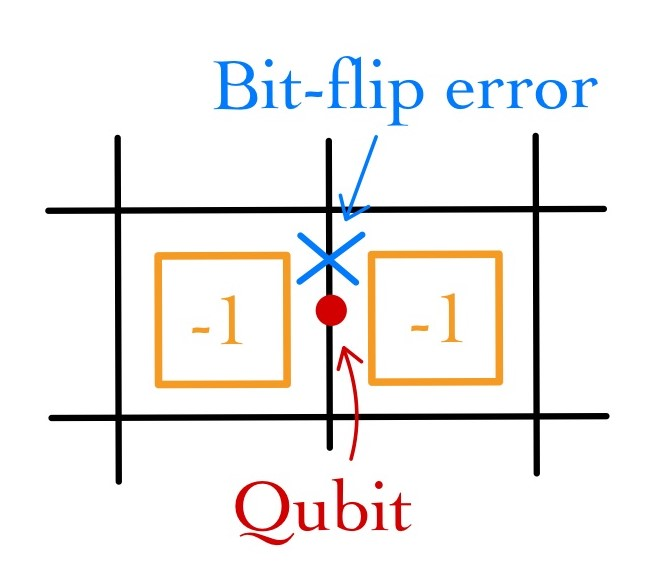
\includegraphics[scale=.32,keepaspectratio]{images/bit_phase_toric_1}} \quad
	\subfloat[][Phase flip error.\label{subfig:bit_phase_toric_2} ]{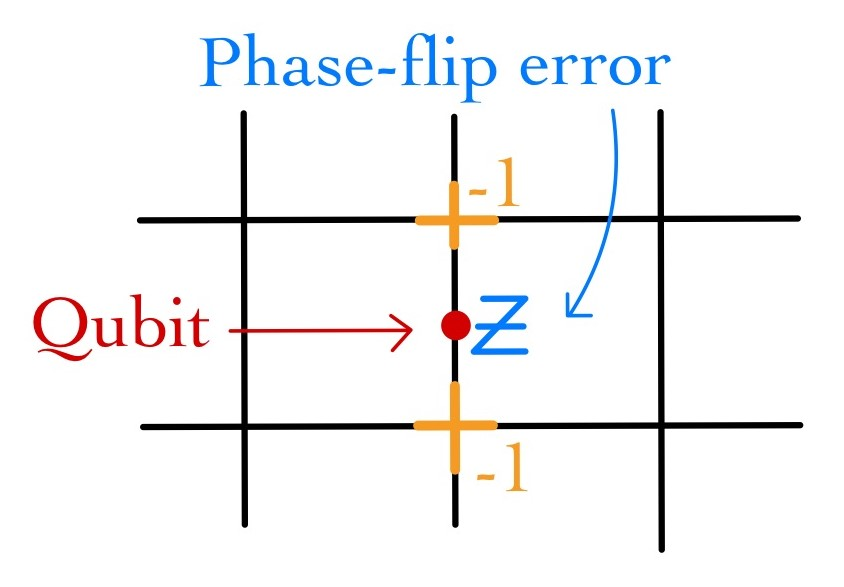
\includegraphics[scale=.32,keepaspectratio]{images/bit_phase_toric_2}} 
	\caption{(\ref{subfig:bit_phase_toric_1}) Esempio di rilevazione di un bit flip error. Solamente le due plaquette (riquadri arancioni) adiacenti all'errore contano perché viene invertito il loro autovalore. (\ref{subfig:bit_phase_toric_2}) Esempio di rilevazione di un phase flip error. Solamente i due vertici (croci arancioni) adiacenti all'errore contano perché viene invertito il loro autovalore.}
    \label{fig:bit_phase_toric}
\end{figure}

\noindent Cominciamo col considerare un \textbf{bit flip error}. Immaginiamo, come in Figura \ref{subfig:bit_phase_toric_1}, di avere un qubit su un link qualsiasi con un errore dato da un \texttt{X-gate}.  In tale situazione solamente le due plaquette adiacenti al link contano: in generale $\comm{X}{A_v} = 0$, ma dato che $B_p = \prod_{j \in p} Z_j$ allora solamente per le due plaquette mostrate avremo $\comm{X}{B_p} \neq 0$. Dato che in particolare si ha $\acomm{X}{B_p} = 0$ per la presenza di uno \texttt{Z-gate} agente sullo stesso sottospazio di $X$ in ciascuna delle due plaquette, allora l'autovalore di questi due $B_p$ su $C$ è diventato $-1$. In questo modo possiamo rilevare un bit flip error misurando l'autovalore di queste due plaquette. Questo significa, in generale, che quando si ha una situazione in cui tutti gli operatori $B_p$ hanno autovalore $+1$ eccetto per due plaquette adiacenti allora sia ha la certezza che è presente un bit flip error nel qubit tra le due. 

\noindent Consideriamo ora un \textbf{phase flip error}. Come evidenziato nella Figura \ref{subfig:bit_phase_toric_2} la situazione è simile alla precedente, ma questa volta l'errore è rappresentato da uno \texttt{Z-gate} su un link: per ogni plaquette avremo $\comm{Z}{B_p} = 0$, ma essendo $A_v = \prod_{i \in v} X_i$ allora per i due vertici adiacenti mostrati si ha $\comm{Z}{A_v} \neq 0$. Come in precedenza, l'errore agisce sul medesimo sottospazio degli operatori $X$ nei due $A_v$, quindi a causa dell'anticommutatore $\acomm{Z}{A_v} = 0$ l'autovalore di questi due vertici sarà $-1$. Esattamente come il caso precedente, quando tutti gli operatori $A_v$ hanno autovalore $+1$ tranne due vertici adiacenti allora si ha la certezza che è presente un phase flip error nel qubit tra i due. 

\noindent Ricapitolando, abbiamo esplicitamente mostrato che gli operatori $A_v$ e $B_p$ agiscono come stabilizers: misurando gli autovalori degli \eqref{A_B} è possibile rilevare direttamente bit flip error e phase flip error. Gli altri errori, ossia la combinazione bit-phase flip, sono semplicemente dati da una combinazione dei casi precedenti. 

\noindent Una delle ragioni principali per cui questo codice di correzione degli errori è così popolare nella letteratura del QC è data dal fatto che sia possibile rilevare e correggere gli errori aggiungendo qubit extra (che chiamiamo anche qui \textbf{ancilla qubits}) nei vertici e nelle facce del reticolo. Tutte le tipologie di qubit presenti nel reticolo (compresi gli ancilla) sono mostrate in Figura \ref{subfig:ancilla_toric_1}. I qubit sui link (pallini rossi pieni) sono i qubit fisici, ossia coloro che codificano l'informazione. Viceversa, i qubit aggiunti sui vertici e al centro delle facce del reticolo (pallini arancio vuoti) sono gli ancilla qubit che hanno lo scopo di effettuare la misurazione e correggere eventuali errori. Chiamiamo \textbf{qubit of type Z} gli ancilla nelle facce perché effettuano la misurazione di $B_p$ sui 4 qubit dei link della plaquette, mentre definiamo \textbf{qubit of type X} gli ancilla presenti nei vertici, i quali similmente effettuano una misurazione di $A_v$ sui 4 qubit dei link entranti in quel vertice.

\noindent Più precisamente, consideriamo la singola plaquette di qubit di Figura \ref{subfig:ancilla_toric_2}. L'ancilla qubit effettua una misurazione dell'operatore $B_p = Z_1 Z_2 Z_3 Z_4$: questa misurazione può essere portata a termine per mezzo del seguente circuito
\begin{center}
    \mbox{
        \Qcircuit @C=2em @R=1em {
            \lstick{\text{Ancilla: }\ket{0}} & \targ & \targ & \targ & \targ & \meter & \rstick{\ket{0}, \ket{1}} \qw \\
            \lstick{1} & \ctrl{-1} & \qw & \qw & \qw & \qw & \qw \\
            \lstick{2} & \qw & \ctrl{-2} & \qw & \qw & \qw & \qw \\
            \lstick{3} & \qw & \qw & \ctrl{-3} & \qw & \qw & \qw \\
            \lstick{4} & \qw & \qw & \qw & \ctrl{-4} & \qw & \qw
        }
    }
\end{center}
L'autovalore del prodotto dei 4 \texttt{Z-gate} di $B_p$ sarà $+1$ o $-1$ a seconda del numero di flip che vengono operati dai \texttt{CNOT-gate}: un numero dispari di stati $\ket{1}$ nei 4 qubit produrrà $B_p = -1$ perché l'ancilla sarà in $\ket{1}$, viceversa un numero pari di $\ket{1}$ vorrà dire $B_p = +1$ perché la misurazione sull'ancilla ha output $\ket{0}$. Misurando quindi lo stato dell'ancilla siamo in grado di stabilire l'autovalore di $B_p$. 

\begin{figure}[!ht]
	\centering	
	\subfloat[][Reticolo di qubit.\label{subfig:ancilla_toric_1} ]{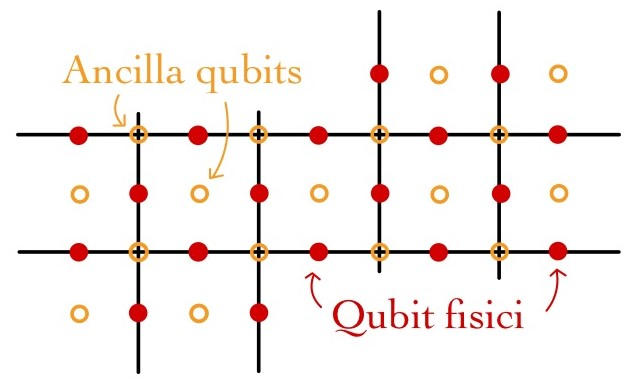
\includegraphics[scale=.45,keepaspectratio]{images/ancilla_toric_1}} \quad
	\subfloat[][Misura di $B_p$.\label{subfig:ancilla_toric_2} ]{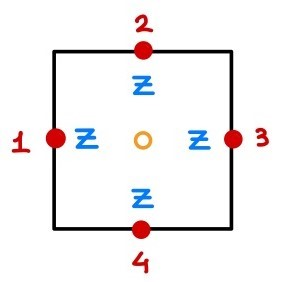
\includegraphics[scale=.45,keepaspectratio]{images/ancilla_toric_2}} \quad
	\subfloat[][Misura di $A_v$.\label{subfig:ancilla_toric_3} ]{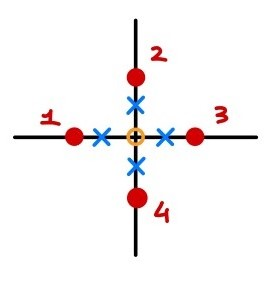
\includegraphics[scale=.45,keepaspectratio]{images/ancilla_toric_3}}
	\caption{Il reticolo è cosparso di qubit fisici (pallini rossi pieni sui link) e di ancilla qubits (pallini arancio vuoti nelle facce e sui vertici). Gli ancilla delle plaquette permettono di effettuare una misurazione dell'autovalore di $B_p$, mentre gli ancilla dei vertici effettuano una misura dell'autovalore di $A_v$.}
    \label{fig:ancilla_toric}
\end{figure}

\noindent In maniera del tutto analoga consideriamo ora il singolo vertice di Figura \ref{subfig:ancilla_toric_3}. È possibile dimostrare che l'ancilla sul vertice effettua una misurazione dell'operatore $A_v = X_1 X_2 X_3 X_4 $ utilizzando un circuito analogo al precedente (vengono solamente inseriti alcuni \texttt{H-gate}): anche in questo caso, una misurazione sullo stato finale dell'ancilla permette di stabilire se l'autovalore è $A_v = +1$ oppure $A_v = -1$. 

\noindent Analizziamo ora gli errori mostrati in Figura \ref{subfig:strange_errors_toric_1}. Come evidenziato anche nella Figura \ref{subfig:bit_phase_toric_1}, la misura nel reticolo di due autovalori $B_p = -1$ corrisponde ad un bit flip error sul qubit tra le due plaquette adiacenti (situazione azzurra in alto nel reticolo). Nonostante la situazione precedente possono avvenire altre tipologie di errori: supponiamo di misurare due autovalori $B_p = -1$ in corrispondenza di due plaquette non adiacenti (si vedano i $-1$ in rosso nelle due facce). Da che cosa sono prodotti errori come i precedenti? Questi non sono altro che il risultato di una serie di bit flip lungo una linea che connette le due plaquette (si veda le "X" in arancio): dato che tutti i link tra le plaquette intermedie hanno cambiato segno due volte a seguito del bit flip, allora per tali facce la misura produce $B_p = +1$, mentre per le plaquette iniziali e finali l'autovalore risulta invertito! Siamo quindi in grado di dare una corretta interpretazione anche di questa tipologia di errore. 

\noindent Perché la natura topologica del codice è così importante? Come possiamo essere certi che l'errore appena spiegato sia dovuto alla linea arancio di bit flip e non, ad esempio, alla linea verde? In principio ogni possibile cammino di \texttt{X-gate} che connette le due plaquette invertite potrebbe dare lo stesso identico errore. Se non sappiamo distinguere quale percorso di \texttt{X-gate} ha causato l'errore, come possiamo correggerlo? Il punto fondamentale è che non importa quale sia il giusto percorso di errori: possiamo correggere gli errori applicando un cammino arbitrario di \texttt{X-gate} lungo un qualsiasi cammino aperto che connette le due plaquette invertite: si tratta quindi di scegliere un cammino di \texttt{X-gate} che connette le due plaquette invertite! Il cammino originale che causa l'errore (non lo conosciamo) più il cammino di \texttt{X-gate} scelto è un operatore banale perché uno compensa l'altro: il percorso finale risultante non è altro che un cammino chiuso nel reticolo duale, quindi la combinazione di errori risulta in un prodotto di \texttt{X-gate} lungo un loop chiuso (Figura \ref{subfig:strange_errors_toric_2})! Dato che, come illustra la Figura \ref{subfig:strange_errors_toric_2}, un qualsiasi prodotto di \texttt{X-gate} su un loop chiuso contraibile può essere scritto come prodotto di $A_p$, allora in analogia alla \eqref{product_Z_closed_loop} avremo
\begin{equation}\label{product_X_closed_loop}
    \prod_{i \in \substack{\text{loop} \\ \text{chiuso}\\ \text{contraibile}}} X_i \equiv \mathbb{I} \, \text{ agendo su } C \, .
\end{equation}

\begin{figure}[!ht]
	\centering	
	\subfloat[][\label{subfig:strange_errors_toric_1} ]{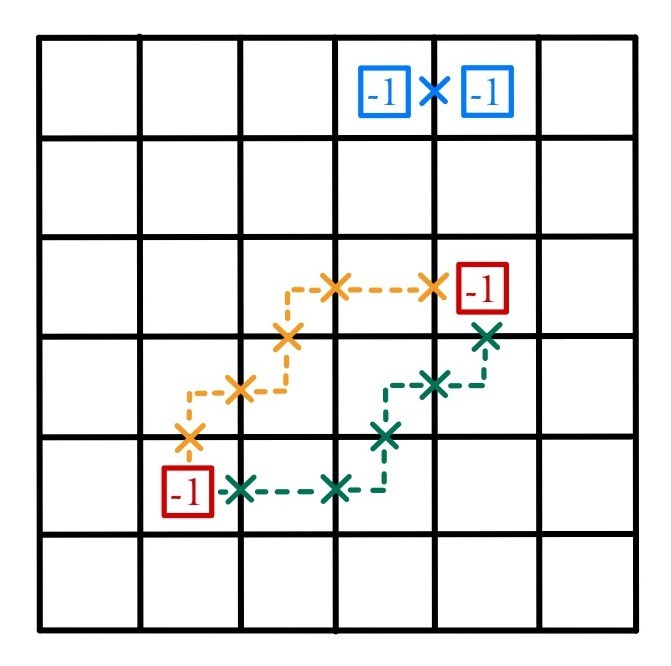
\includegraphics[scale=.38,keepaspectratio]{images/strange_errors_toric_1}} \qquad
	\subfloat[][\label{subfig:strange_errors_toric_2} ]{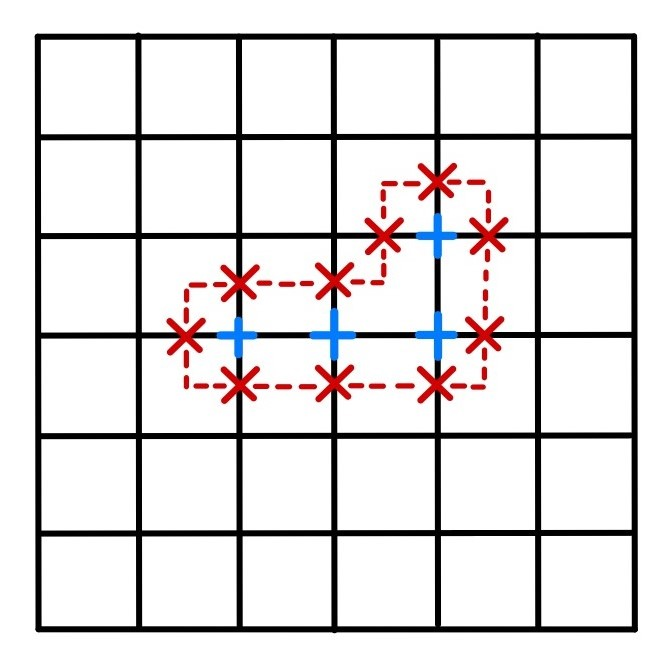
\includegraphics[scale=.38,keepaspectratio]{images/strange_errors_toric_2}}
	\caption{(\ref{subfig:strange_errors_toric_1}) La misura di due autovalori $B_p = -1$ in corrispondenza di due plaquette non adiacenti (facce in rosso) può essere causata da una concatenazione di bit flip errors lungo un cammino che connette le due plaquette. Per correggere tale errore basta applicare un percorso di \texttt{X-gate} che connette le due plaquette. (\ref{subfig:strange_errors_toric_2}) Un prodotto di \texttt{X-gate} su un loop chiuso nel reticolo duale è equivalente ad un prodotto di operatori $A_v$ (vertici azzurri), i quali hanno contributo banale su $C$.}
    \label{fig:strange_errors_toric}
\end{figure}

\noindent Ricapitolando: un cammino chiuso di \texttt{X-gate} nel reticolo duale può sempre essere visto come prodotto di tutti i vertici (operatori $A_v$) contenuti nel loop; ogni $A_p$ inserisce un \texttt{X-gate} sui link esterni mentre, grazie a $X^2 = \mathbb{I}$, nulla accade nei link interni comuni ai vertici. Dato che su $C$ tutti gli $A_p$ hanno autovalore $+1$, allora i loop chiusi di \texttt{X-gate} nel reticolo duale sono omotopi a zero, ossia sono l'operatore banale (identità). 

\subsection{Interpretazione in meccanica statistica}
Esiste una curiosa interpretazione del toric code alla luce della meccanica statistica considerando un reale modello di spin quantistici. Supponiamo un reticolo in cui, su ogni link, è possibile avere uno spin quantistico (up o down). In un tale sistema l'hamiltoniana è data da 
\begin{equation}\label{hamilt_toric}
    H = - J \sum_v A_v - J \sum_p B_p \, , \qquad J > 0 \, .
\end{equation}
Come mostra la Figura \ref{subfig:stat_mec_toric_1}, l'interazione degli spin avviene in due modi: interagiscono i 4 spin in un vertice (prima somma in $H$) oppure i 4 spin di una plaquette (seconda somma in $H$). Qual è lo stato (o gli stati) di minima energia? I ground state corrispondono a tutte quelle situazioni in cui gli autovalori sono $A_v = B_p = +1$ per ogni vertice e plaquette del reticolo. In un'interpretazione di questo tipo i 4 stati logici $\ket{\overline{00}}$, $\ket{\overline{01}}$, $\ket{\overline{10}}$ e $\ket{\overline{11}}$ (con autovalori $A_v = B_p = +1$) del QC sono mappati nei ground state dell'hamiltoniana \eqref{hamilt_toric}; viceversa gli errori nel reticolo corrispondono a delle eccitazioni, ossia a delle configurazioni in cui almeno un autovalore di $A_v$ e/o $B_p$ è uguale a $-1$. 

\begin{figure}[!ht]
	\centering	
	\subfloat[][\label{subfig:stat_mec_toric_1} ]{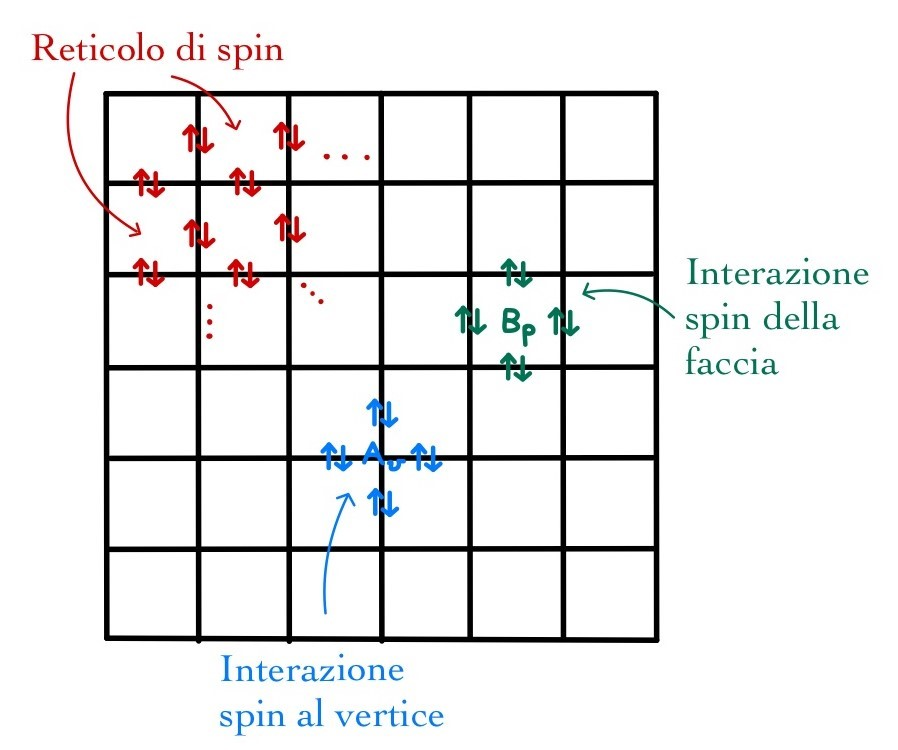
\includegraphics[scale=.35,keepaspectratio]{images/stat_mec_toric_1}} \quad
	\subfloat[][\label{subfig:stat_mec_toric_2} ]{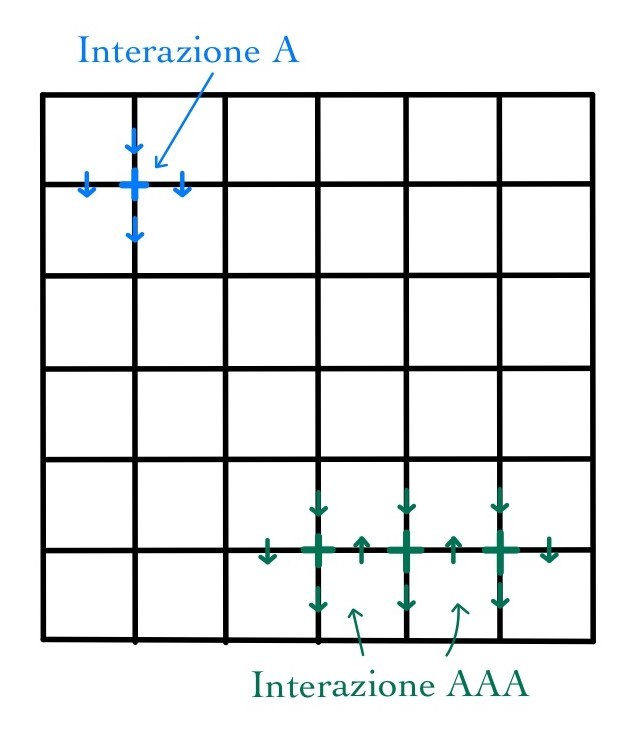
\includegraphics[scale=.35,keepaspectratio]{images/stat_mec_toric_2}}
	\caption{(\ref{subfig:stat_mec_toric_1}) L'analogo sistema in meccanica statistica del toric code è costituito da un reticolo di spin in cui questi ultimi possono interagire in un vertice oppure in una plaquette. (\ref{subfig:stat_mec_toric_2}) Se si espande la produttoria in \eqref{logical_00} si hanno diverse interazioni di spin a causa delle combinazioni degli operatori $A_v$.}
    \label{fig:stat_mec_toric}
\end{figure}

\noindent Dal punto di vista dei singoli spin lo stato \eqref{logical_00} è estremamente complicato perché è uno stato molto entangled. Se si espande la produttoria in $\ket{\overline{00}}$ si ottengono dei termini del tipo $\mathbb{I} + A + AA + AAA + \ldots$, quindi avvengono diverse interazioni: come illustra la Figura \ref{subfig:stat_mec_toric_2}, il singolo operatore $A$ agisce sul vertice e inverte i 4 spin (in blu in alto a sinistra dove gli spin $\uparrow$ sono diventati $\downarrow$); gli operatori della forma $AAA$, invece, creano un loop di spin capovolti nel reticolo originale (si vedano i tre vertici in basso in verde). In totale la produttoria in \eqref{logical_00} produce una sovrapposizione lineare di tutti i possibili loop costituiti da spin invertiti: c'è entanglement tra tutti gli spin del reticolo, persino tra quelli più distanti. 

\noindent Che cosa sono gli errori in QC? Non sono altro che operatori che agiscono sui link del reticolo: ad esempio se si pensa ad un singolo bit flip error (\texttt{X-gate} su un link) allora esso cambia autovalore agli operatori $B_p$ delle placchette adiacenti (si veda la Figura \ref{subfig:bit_phase_toric_1}); similmente quando si ha un phase flip error (Figura \ref{subfig:bit_phase_toric_2}), allora lo \texttt{Z-gate} sul link corrotto cambierà autovalore ai due operatori $A_v$ adiacenti. 

\noindent Data l'hamiltoniana \eqref{hamilt_toric}, agli errori nel QC corrispondono delle eccitazioni nel sistema di spin: avremo una variazione di energia $\Delta E_z = 2 J$ per il singolo phase flip e una variazione di $\Delta E_x = 2 J$ per il singolo bit flip. In teoria della materia condensata questi stati eccitati corrispondono alle cosiddette \textbf{quasiparticles}. In questo contesto ne esistono di due tipologie: le quasiparticle \textbf{elettriche}, a seguito dell'errore causato da $Z$ e le quasiparticle \textbf{magnetiche}, generate dall'errore di $X$; entrambe hanno la medesima energia e  vedremo nelle prossime sezioni che presentano alcune proprietà strane e insolite. Dato che per ogni errore (bit flip o phase flip) si hanno due autovalori $-1$ ($A_v = -1$ per $Z$ e $B_p = -1$ per $X$) allora è come se potessimo associare due paia di quasiparticle: 2 elettriche e 2 magnetiche. 

\noindent Una delle proprietà più insolite (vedremo) è la seguente: se si considera una quasiparticle elettrica e la si muove attorno ad una quasiparticle magnetica ritornando poi al punto di origine allora, a seguito della QM, si origina una fase: questo fenomeno può essere interpretato come un doppio scambio di particelle; per tale ragione questa particolare tipologia di particelle costituiscono un perfetto "toy model" per i cosiddetti \textbf{anyons} (diffusi in letteratura nella teoria della materia condensata). Queste particolari quasiparticle, presenti unicamente in sistemi bidimensionali, sono simili a particelle che presentano una statistica frazionaria, ossia non sono né bosoni né fermioni!